\label{ch:intro}

% Other research reactor applications: support energy production, space discovery, etc ...
% iaea-research: https://www.iaea.org/sites/default/files/18/05/research-reactors-purpose-and-future.pdf
% https://world-nuclear.org/information-library/non-power-nuclear-applications/radioisotopes-research/research-reactors.aspx
% https://www-pub.iaea.org/MTCD/Publications/PDF/Pub1627_web.pdf

% Research Reactors intro
Research reactors are nuclear reactors that work as neutron and gamma sources for research and various applications.
In contrast to \glspl*{NPP}, they are not used to produce heat for electricity generation, and consequently, they are smaller.
Their power ratings are smaller too compared to \glspl*{NPP}, typically ranging from zero up to 200 MWth \cite{iaea-research}.
Smaller sizes and power ratings make them less complex with simpler systems and designs that make them well suited for education and training of reactor operators, radiation protection personnel, students, and researchers.

% Uses and purposes
Research reactors enable a vast range of uses and purposes, including scientific research, material testing, and radioactive material production.
% scientific research
An example of scientific research is the utilization of thermal and cold neutron facilities, as in the Argentinian reactor RA-10 shown in Figure \ref{fig:intro-1}, to study the structure of matter via neutron scattering.
Knowing the internal structure of matter helps understand the macroscopic properties of materials.
By performing neutron scattering, biologists understand the repair and decay processes in the bones, physicists create more powerful magnets, and neuron experts study proteins in the brain, just to mention a few areas of research \cite{iaea-research}.

\begin{figure}[htbp!] % or H
  \centering
  \begin{subfigure}[b]{0.49\textwidth}
    \centering
    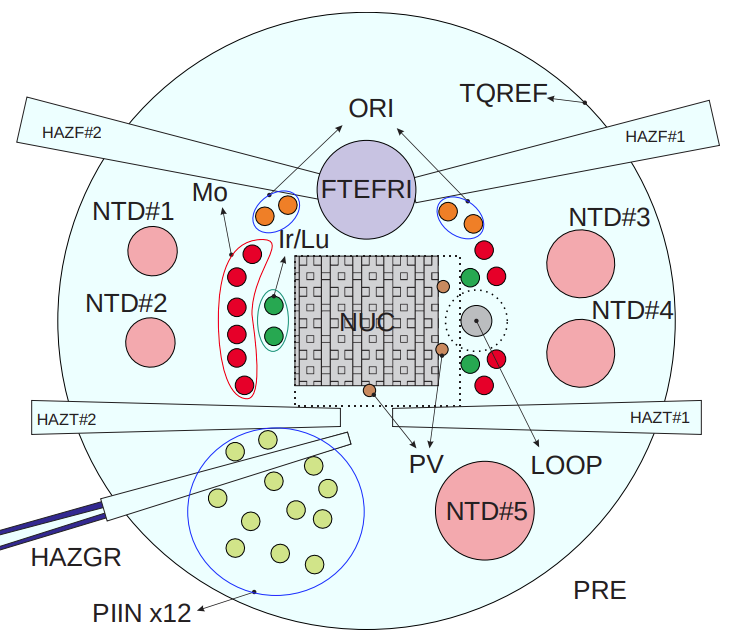
\includegraphics[width=0.95\textwidth]{figures/RA-10}
    \caption{Scientific research in the Argentinian reactor RA-10 \cite{ra10}.}
  \end{subfigure}
  \hfill
  \begin{subfigure}[b]{0.49\textwidth}
    \centering
    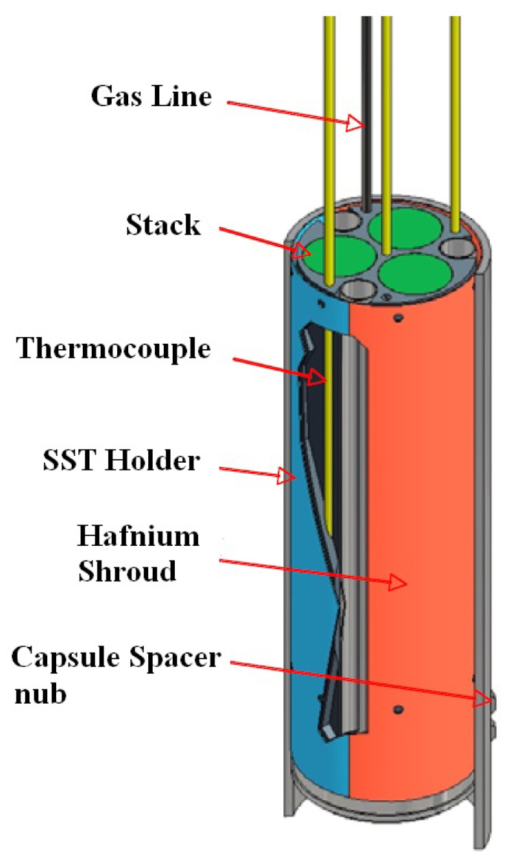
\includegraphics[width=0.50\textwidth]{figures/agr1}
    \caption{Material testing of the \gls*{AGR1} capsule \cite{sterbentz_agr1_2018}.}
  \end{subfigure}
  \hfill
  \caption{Examples of research reactor uses.}
  \label{fig:intro-1}
\end{figure}

% material testing
Material characterization and testing is a technique to study the effects of radiation on the material properties.
Neutrons induce changes in the materials' structure, making them fragile, elastic or hardened, swell, crumble, change their composition, release gas, etc.
Moreover, research reactors test advanced reactor fuel which supports their design optimization.
The \gls*{AGR1} experiment \cite{sterbentz_agr1_2018}, shown in Figure \ref{fig:intro-1}, was an irradiation test to provide performance data during normal operation of the fuel utilized in \glspl*{HTGR}.

% radioactive material production
Another frequent use of research reactors is radioactive material production, which encompasses three main applications: neutron activation analysis, neutron transmutation doping, and radioisotope production for medicine.
Figure \ref{fig:intro-2} shows some examples of these applications.
% neutron activation analysis
% https://www.iaea.org/sites/default/files/18/05/research-reactors-purpose-and-future.pdf
Neutron activation analysis is a technique to measure the elemental composition of water, air, soil, rocks, etc.
The samples are irradiated and by studying their characteristic gamma emissions it is possible to identify trace elements in the range of parts per billion.
% neutron transmutation
Neutron transmutation doping changes silicon properties, making it conductive, and the electronics industry highly benefits from this application for chip production.
% radioisotopes
Finally, the medical field utilizes radioisotopes for diagnosing and treating health conditions like cancer and cardiovascular diseases.
For example, technetium-99m comes from the decay of molybdenum-99, and its primary use is diagnostic imaging \cite{mattar_exploring_2019}.


\begin{figure}[htbp!] % or H
  \centering
  \begin{subfigure}[b]{0.45\textwidth}
    \centering
    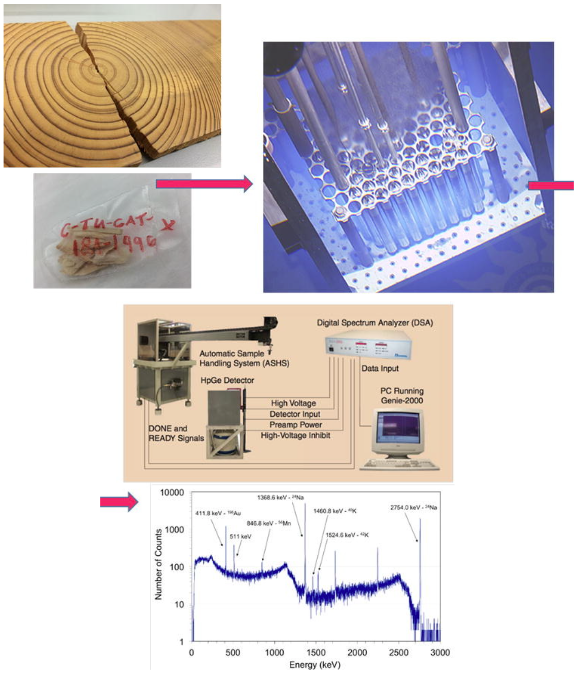
\includegraphics[width=0.75\textwidth]{figures/neutron-activation}
    \caption{Neutron activation analysis \cite{neutron-activation}.}
  \end{subfigure}
  \hfill
  \begin{subfigure}[b]{0.53\textwidth}
    \centering
    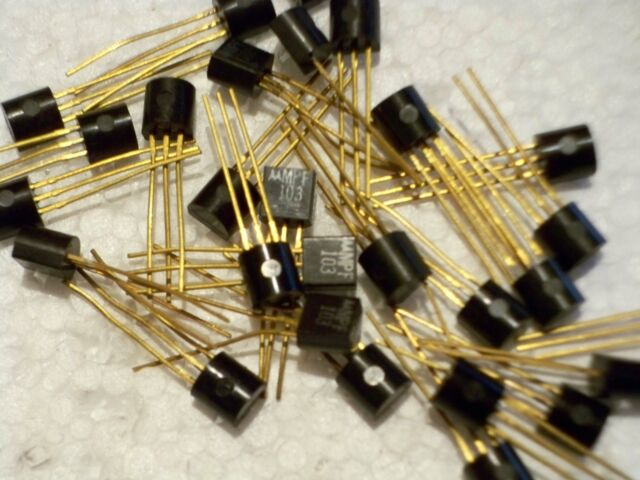
\includegraphics[width=0.95\textwidth]{figures/neutron-transmutation}
    \caption{Neutron transmutation doping.}
  \end{subfigure}
  \hfill
  \begin{subfigure}[b]{0.49\textwidth}
    \centering
    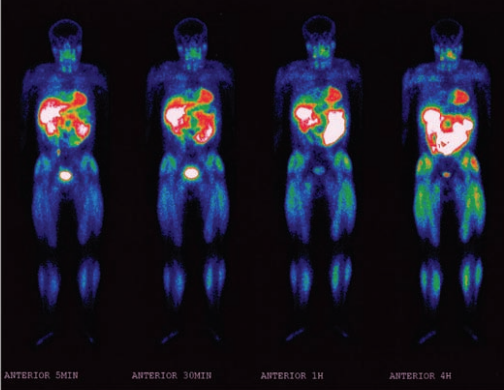
\includegraphics[width=0.95\textwidth]{figures/tc-99}
    \caption{Medicine applications. Whole body scan in a human administered with Tc-99m \cite{tc99m}.}
  \end{subfigure}
  \caption{Examples of applications of radioactive material production.}
  \label{fig:intro-2}
\end{figure}

% Some more: https://www.iaea.org/newscenter/news/exploring-research-reactors-and-their-use#:~:text=Research%20reactors%20are%20small%20nuclear%20reactors%20that%20are%20primarily%20used,and%20used%20to%20generate%20electricity.
% And some more: https://www.antinternational.com/docs/samples/FM/11/ZIRAT23_STR_Material_Test_Reactors_and_other_Irradiation_Facilities_Sample.pdf


\section{Motivation}

% https://www-pub.iaea.org/MTCD/Publications/PDF/Pub1321_web.pdf
% https://www-pub.iaea.org/MTCD/Publications/PDF/PUB1981_web.pdf

% Transition
The \gls*{IAEA} Safety Fundamentals state that the main safety objective in all nuclear installations is to protect people and the environment by establishing an effective defense against radiological hazards \cite{iaea-safety2}.
Fulfilling this objective requires the quantification of the risk of radiation release to the environment that may arise from a nuclear reactor.
Safety analyses assess the performance of the reactor against a broad range of operating conditions and demonstrate the prevention of radioactive material releases.
They can also identify hidden weaknesses and guide design improvements.
Although research reactors have a much smaller size and power than \glspl*{NPP}, safety analyses are still required.

Research reactor safety analyses demonstrate to the regulatory body the contribution of the operational procedures to the prevention and mitigation of accidents.
However, these analyses focus on the reactor core and disregard a thorough examination of the experiments.
This work defines an experiment as any device utilized in any of the aforementioned research reactor applications.
The development of experiment safety analyses is paramount to ensure safe experiment activities during any planned or unplanned events.
Accordingly, the \gls*{IAEA} recommends that experiment safety analyses include a list of possible hazards and any operational limits, such as maximum temperatures and pressures \cite{noauthor_safety_2012}.

% The problem
Research reactors enable the irradiation of a wide variety of experiments, which may have different combinations of shapes and materials.
Therefore, experiments tend to be unique, requiring independent calculations and the development of safety analyses on a case-by-case basis.
In consequence, the development of individual analyses often tends to be effort- and time-consuming.
% Also need for a unified workflow --> otherwise it is error prone
For instance, the initial experiment definition, design, and fabrication of a simple static capsule experiment for the \gls*{ATR} takes six months \cite{inl_advanced_2009}.
Nevertheless, using previously analyzed configurations can shorten this process.
%
Another example is the \gls*{NSUF} of the \gls*{HFIR}, wherein the experiment proposal review process requires the experiment materials and parameters to fall within the bounds of previously approved experiments \cite{hfir}.
For experiments falling outside these bounds, additional procedures are required, translating to longer processing times.
This reinforces the idea that using previous knowledge can expedite the process.

The present work supports the development of experiment safety analysis, and, to narrow down the scope of the analysis, it studies the bounding event - i.e., the most thermally challenging scenario that an experiment could undergo within the design basis accidents, a channel draining event.
The section on the left of Figure \ref{fig:diagra1} shows the standard workflow for the evaluation of the experiment state during the bounding event.
The workflow consists of a delayed heating calculation and the \gls*{CFD} modeling of the experiment.
The delayed heating calculation relies on a three-step process.
First, a neutron-transport simulation determines the flux distribution.
Second, a depletion simulation determines the material composition, decay rates, and photon energy distribution.
Third, a photon-transport simulation estimates the energy deposition in the experiment.
The subsequent run and exchange of information between these steps and the CFD simulation is commonly carried out manually by the lack of a streamlined workflow.
In consequence, the development of experiment safety analyses tends to not only be effort- and time-consuming, but also error-prone, as each of these steps introduces an instance for an error to occur.

\begin{figure}[htbp!]
  \centering
  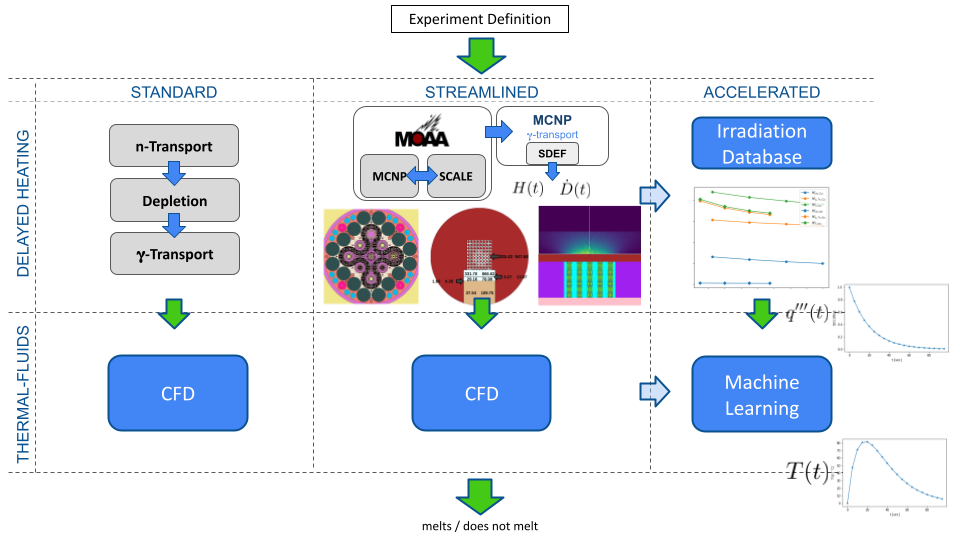
\includegraphics[width=0.99\textwidth]{figures/diagram}
  \caption{Calculation procedure to determine experiment state during a channel draining event.}
  \label{fig:diagra1}
\end{figure}


\section{Objectives}

% What is the main objective?
The objective of this Ph.D. thesis is to reduce the effort and time invested in the development of experiment safety analyses and to lower the chance of errors.
This objective can be separated into two parts.
The first part streamlines the calculation workflow, and the second part accelerates it by integrating previous knowledge into the process.
The section in the center of Figure \ref{fig:diagra1} provides a visual representation of the streamlined workflow that fulfills the requirements of the first part of the objective.
The streamlined workflow automates the transfer of information within the delayed heating calculation workflow as well as to the CFD simulation.
This objective can be organized into the following main subtopics.

% Secondary objectives
\textbf{Study the capsule's integrity during a channel draining event.}
Specifically, this work develops modeling capabilities to quickly predict the outcome of the bounding event on the experiment  and if it leads to a radioactive material release.
Additionally, the range of applicability of these capabilities should encompass any experiment material composition.
The present work considers the melting of the capsule encasing the experiment as the threshold for the radioactive material release.
The accident progression considers the following events: the safety system stops the fission reactions in the core, the experiment channel loses all the coolant, air fills up the remaining space, and the resulting natural circulation of air cools down the experiment.
The study takes a conservative approach and considers that the channel is drained instantly after shutdown.
% The following list of objectives expands on this goal.

% Thermal-fluids model
\textbf{Create a CFD model of the experiment.}
Effective heat removal prevents overheating damage that may lead to a radioactive material release.
Quantifying the capsule cooling requirements, and hence ensuring the capsule's integrity, requires the development of a thermal-fluids model to accurately predict the capsule temperature.

% Decay heat calculation
\textbf{Develop delayed heating calculation capabilities.}
In an operating reactor, there is an equilibrium between the generated and removed heat.
After reactor shutdown, the radioactive materials continue to decay and release energy.
This energy is deposited across the reactor, and it is the cause of the delayed heating.
The assessment of the energy deposited in the experiment provides the thermal-fluids model with the volumetric heat source to accurately calculate the capsule temperature.
The delayed heating calculation workflow can not only calculate the heating in the reactor experiments but also in reactor structures, which is a feature that will be demonstrated.

% Shutdown dose rate calculation
\textbf{Shutdown dose rate calculations.}
After the experiment has been extracted from the reactor, the ongoing decay exposes workers and equipment in the surroundings to radiation dose.
Safety analyses require the quantification of this dose.
A value-added of the delayed heating calculation is the shutdown dose rate, which removes the need for additional workflow for radiation dose rates and will be demonstrated for the post-irradiation examination of an experiment.
% The calculation of the shutdown dose rate will be demonstrated for the post-irradiation examination of AGR-1, a TRISO-fueled experiment in ATR.

The workflow described above streamlines the calculation procedure of experiment safety analyses.
The section on the right of Figure \ref{fig:diagra1} shows the accelerated workflow that intends to decrease the calculation burden significantly, which fulfills the requirement of the second part of this Ph.D. thesis objective.
The first part of the accelerated calculation is the delayed heating in the experiment, which relies on the use of the delayed heating calculation of the streamlined workflow.
This step entails the creation of a generic material irradiation database with which it is possible to estimate the delayed heating of experiments of arbitrary material composition.
The second component of the accelerated calculation is the determination of the bounding event outcome.
This part uses the CFD calculation of the streamlined workflow to train and test several machine learning algorithms and examine their applicability to further lower the calculation burden.
This objective can be organized into the following main subtopics.

% Additionally, the proposed methodology includes the creation of a generic material irradiation database to further decrease the calculation burden.
% Furthermore, this work examines the applicability of machine learning algorithms to reduce this burden even further.

\textbf{Generate a delayed heating database.}
Research reactors fulfill the radioisotope needs from multiple fields.
Consequently, the range of materials that form the experiments is vast.
For example, the medical field requires a supply of cobalt-60, yttrium-90, molybdenum-99, iodine-131, and iridium-192.
Therefore, this work aims to create a model extensible to all possible irradiated materials.
The creation of the database involves utilizing the delayed heating calculation workflow to obtain the delayed heating for experiments composed of individual chemical elements.
% Nevertheless, an experiment usually comprises a mix of different elements.
% This work creates a method for calculating the delayed heating of an experiment as a combination of the delayed heating of the individual elements that are part of it.
This work creates a method that uses such a database to calculate the delayed heating in experiments of arbitrary composition.
This method will be verified for selected materials.

% Surrogate model
\textbf{Build a data-based model.}
The thermal-fluids model enables the determination of the capsule temperature for an experiment.
However, running the thermal-fluids model for each individual experiment is computationally expensive.
The data-based model utilizes machine learning to further lower the computational burden and quickly predict the accident outcome.
The present work compares their performance and examines their applicability to experiment safety analysis.
Ultimately, the data-based model aims to predict if the capsule melts for any experiment material composition, provided its thermal properties are known.
Two main strategies were chosen.
The first strategy relies on classification methods to predict the state of the capsule.
The second approach uses deep-learning to predict the capsule temperature evolution.

% Demonstrate in ATR
\textbf{Demonstrate the modeling capability by its application to ATR.}
The fulfillment of this thesis' objectives is complete with the application, demonstration, and verification of the presented developments on a full-size research reactor.
This thesis focuses on the \gls*{ATR}, and this objective consists of the following steps: create a detailed delayed heating database for an ATR experiment, tailor the thermal-fluids model to the experiment, and train and test a data-based model specific to the experiment.


\section{Outline}

This thesis describes the motivation, objectives, methodology, results, and conclusions towards the advancement of the state-of-the-art of research reactor experiment analysis.
The remainder of this document is organized as follows.
Chapter \ref{ch:lit} presents a literature review organizing and summarizing previous relevant work to this thesis.
Chapter \ref{ch:delayedheat} describes the delayed heating calculation workflow and demonstrates it for  multiple examples.
Chapter \ref{ch:sdr} focuses on the shutdown dose rate calculation workflow and several demonstration cases.
Chapter \ref{ch:database} introduces the generic material irradiation database method, and its verification with selected materials commonly used in nuclear engineering.
Chapter \ref{ch:tf} describes the utilized machine learning algorithms, the implementation strategies, and the train and test of different exercises.
Chapter \ref{ch:concl} summarizes the contributions of this thesis to the nuclear engineering field.

%%%% Figures
% \begin{figure}[htbp!]
% 	\centering
% 	\includegraphics[height=4.0cm]{figures/triso}
% 	\caption{Drawing of a TRISO fuel particle. Image reproduced from \cite{hales_multidimensional_2013}.}
% 	\label{fig:triso}
% \end{figure}

% \begin{figure}[htbp!]
%     \centering
%     \subfloat[Reactor layout. Image reproduced from \cite{barre_gas-cooled_2010}. \label{fig:fsv-a}]{
%         \includegraphics[width=0.40\textwidth]{figures/fsv-core}
%     }
%     \subfloat[Fuel assembly. Image reproduced from \cite{melese_thermal_1984}. \label{fig:fsv-b}]{
%         \includegraphics[width=0.41\textwidth]{figures/fsv-assembly}
%     }
%     \hfill
%     \caption{Fort St. Vrain Generating Station.}
%     \label{fig:fsv}
% \end{figure}
